%---------------------------------------------------------------------------------------------------
% Modellierung
%---------------------------------------------------------------------------------------------------
\section{Modellierung}

Das Experiment besteht grob aus drei Phasen:
\begin{itemize}
  \item Aufstieg im Ballon
  \item Absprung und freier Fall
  \item Gebremster Fall am Fallschirm und Landung
\end{itemize}
Der Aufstieg wird im Rahmen dieser Arbeit nicht weiter betrachtet.
Interessanter ist der Fall - vor allem der ungebremste Abschnitt von Absprung bis zum Öffnen des Fallschirms.
Um dies zu simulieren, müssen relevante Kräfte und Größen berücksichtigt werden. %identifiziert und modelliert werden.

Seitenwinde und mögliche Rotation werden ignoriert.
Als Masse für Springer und Ausrüstung werden $140kg$ angeommen.
Auf den Springer und seine Ausrüstung wirken lediglich zwei Kräfte:
\begin{description}
  \item[$F_g$] Zur Erde hin wirkt die Gravitation.
  \item[$F_L$] Bremsend wirkt der Luftwiderstand, der sich bei Öffnen des Fallschirms massiv erhöht.
\end{description}

Die ausschlaggebenden Größen werden im Folgenden beschrieben.

\subsection{Gravitation}
Die Gravitation wirkt zwischen dem Springer und der Erde.
Allgemein wird hier das newtonsches Gravitationsgesetz angewendet.
\begin{equation}
F_g=G \frac{m_1 m_2}{r^2}
\end{equation}
Dabei ist $G$ die Gravitationskonstante $66,7384\times 10^{-12} \frac{m^3}{kg\ s^2}$, $m_1$ und $m_2$ die beteiligten Massen und $r$ deren Abstand.
Bis auf $r$ (der Springer bewegt sich ja auf die Erde zu) sind hier alle Größen konstant.
$r$ ist dabei gleich dem Radius der Erde plus der Höhe des Springers \vgl Abb.~\ref{fig:gravitation}.
\begin{figure}[h]
  \centering
  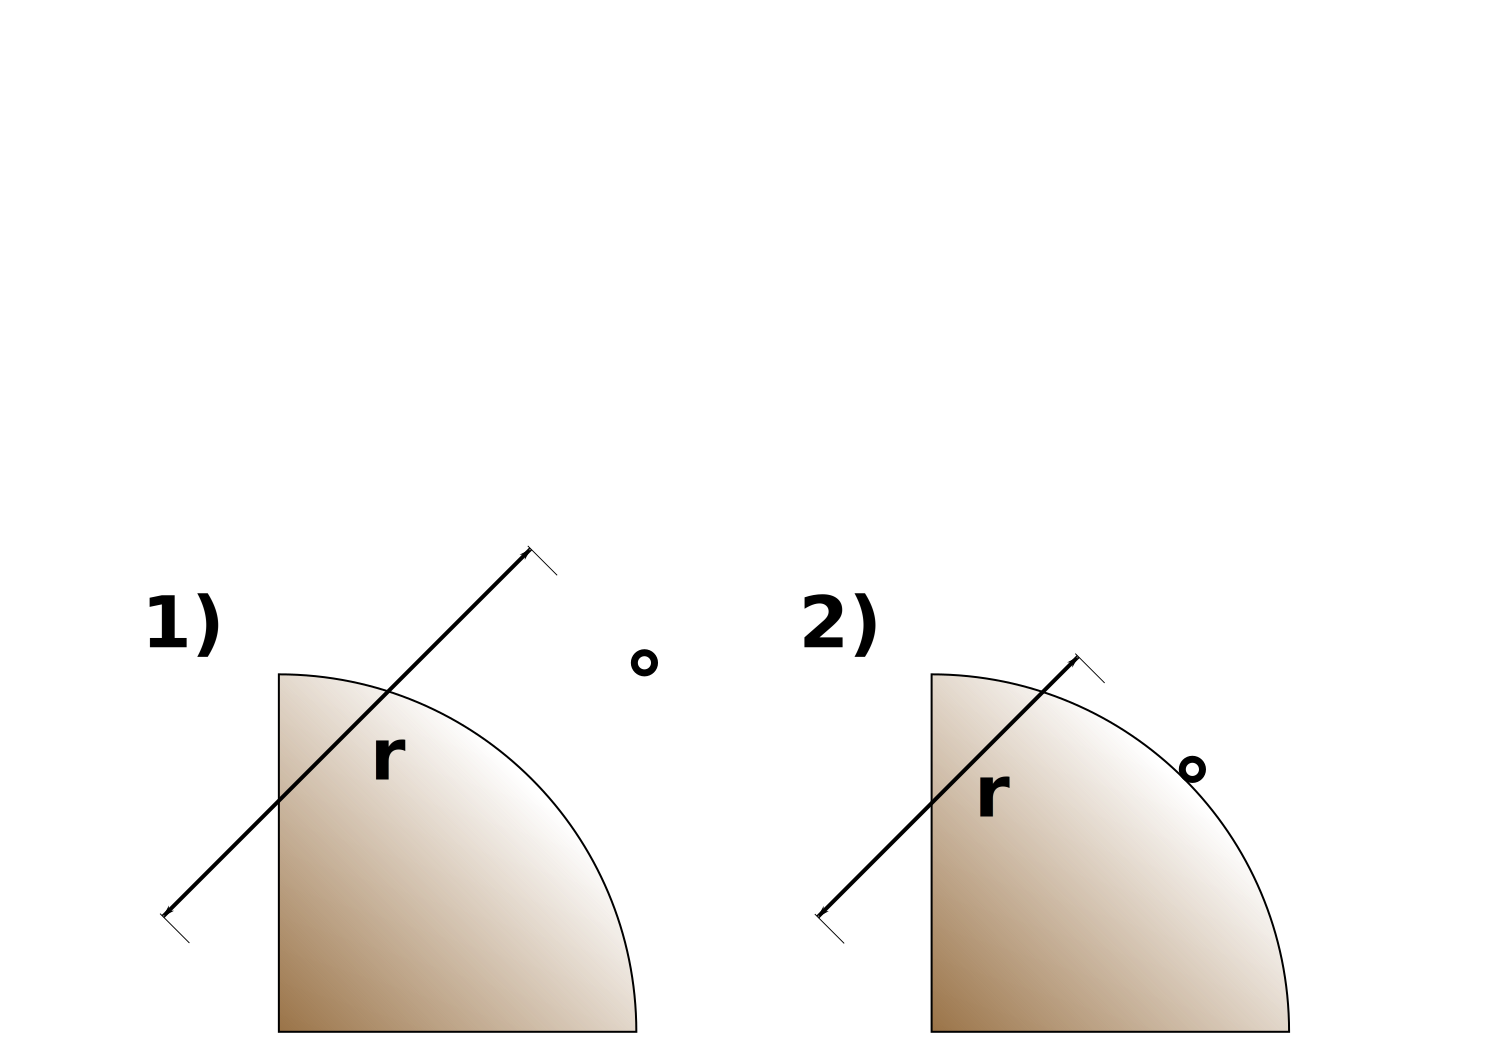
\includegraphics[width=0.5\textwidth]{gravitation}
  \caption{$r$ bei 1) Absprung und 2) Landung}
  \label{fig:gravitation}
\end{figure}

Als Erdradius wird der Äquatorradius $R_A=6.378.137m$ angenommen, als Masse des Springers $m_1=140kg$, als Masse der Erde $m_2=5,9736\times 10^{24}kg$.
Die Kraft, die auf den Springer auf Erdniveau herrscht beträgt
\begin{eqnarray}
F_{g0} &=& 66,7384\cdot 10^{-12} \frac{140\cdot 5,9736\cdot 10^{24}}{6.378.137^2} \\
 &=& 1.372 N \nonumber
\end{eqnarray}
Die Challenger zerbrach in $15km$ Höhe, der Sprung Baumgartners erfolgte aus knapp $40km$.
Um den Effekt der Höhenänderung möglichs deutlich zu zeigen wird als zweiter Wert die Gravitationskraft in $40km$ Höhe berechnet.
\begin{eqnarray}
F_{g1} &=& 66,7384\cdot 10^{-12} \frac{140\cdot 5,9736\cdot 10^{24}}{\left(6.378.137 + 40.000\right)^2} \\
 &=& 1.354,9 N \nonumber
\end{eqnarray}
Die Gravitationkraft nimmt in Absprunghöhe gegenüber der auf Erdniveau herrschenden um knapp $2\%$ ab.

\subsection{Luftwiderstand}
Die Atmosphäre ist keine homogene Gasblase.
Sie ist komplexer aufgebaut.
Für die Simulation sind dabei die Temperatur und die Dichte in der jeweiligen Höhe von Bedeutung.

\subsubsection{Dichte}
Mit steigender Höhe nimmt die Dichte ab, da die darüberliegendes Gassäule kürzer wird.

\subsubsection{Temperatur}

\subsection{Strömungswiderstand}

\subsubsection{Überschallflug}
